\chapter[Ejemplos del asistente conversacional]{Ejemplos de interacción con el asistente conversacional}
\label{ap:llm-ejemplos}

Este apéndice complementa los ejemplos del capítulo de resultados
(sección~\ref{sec:res-ia-llm}) con una muestra por cada tipo de maniobra que el asistente
resuelve, para ilustrar la variedad de peticiones que admite. Las transferencias entre
órbitas y el mantenimiento orbital ya se ilustraron en el cuerpo del documento; se recogen
aquí las restantes. Cada caso se acompaña de dos figuras: la conversación en la que el
asistente interpreta la petición e invoca la herramienta ---un agente de \gls{RL} o un
solucionador clásico---, y la figura que él mismo genera como respuesta.

% ---------------------------------------------------------------------------
\section{Transferencia con cambio de plano}
\label{ap:llm-cambioplano}

El asistente reconoce cuándo la petición implica, además de subir de órbita, girar el plano
orbital, y recurre al agente tridimensional, que devuelve el coste y el reparto del giro
entre los dos impulsos (figura~\ref{fig:ap-llm-cambioplano-chat}). La
figura~\ref{fig:ap-llm-cambioplano-fig} muestra la representación tridimensional que genera a
continuación, en la que se aprecia la inclinación de la órbita final.

\begin{figure}[htbp]
  \centering
  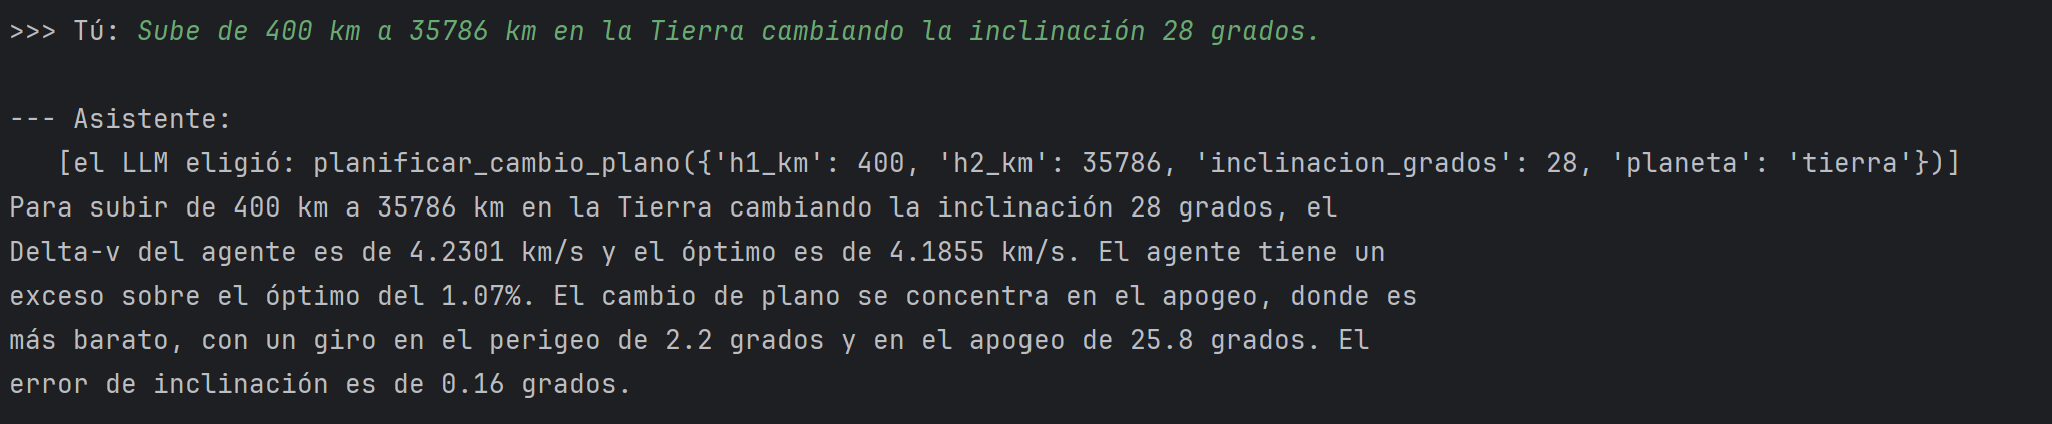
\includegraphics[width=0.9\textwidth]{tex/imagenes/llm_chat_cambio_plano.png}
  \caption{Conversación: el asistente planifica una transferencia con cambio de plano.
  Elaboración propia.}
  \label{fig:ap-llm-cambioplano-chat}
\end{figure}

\begin{figure}[htbp]
  \centering
  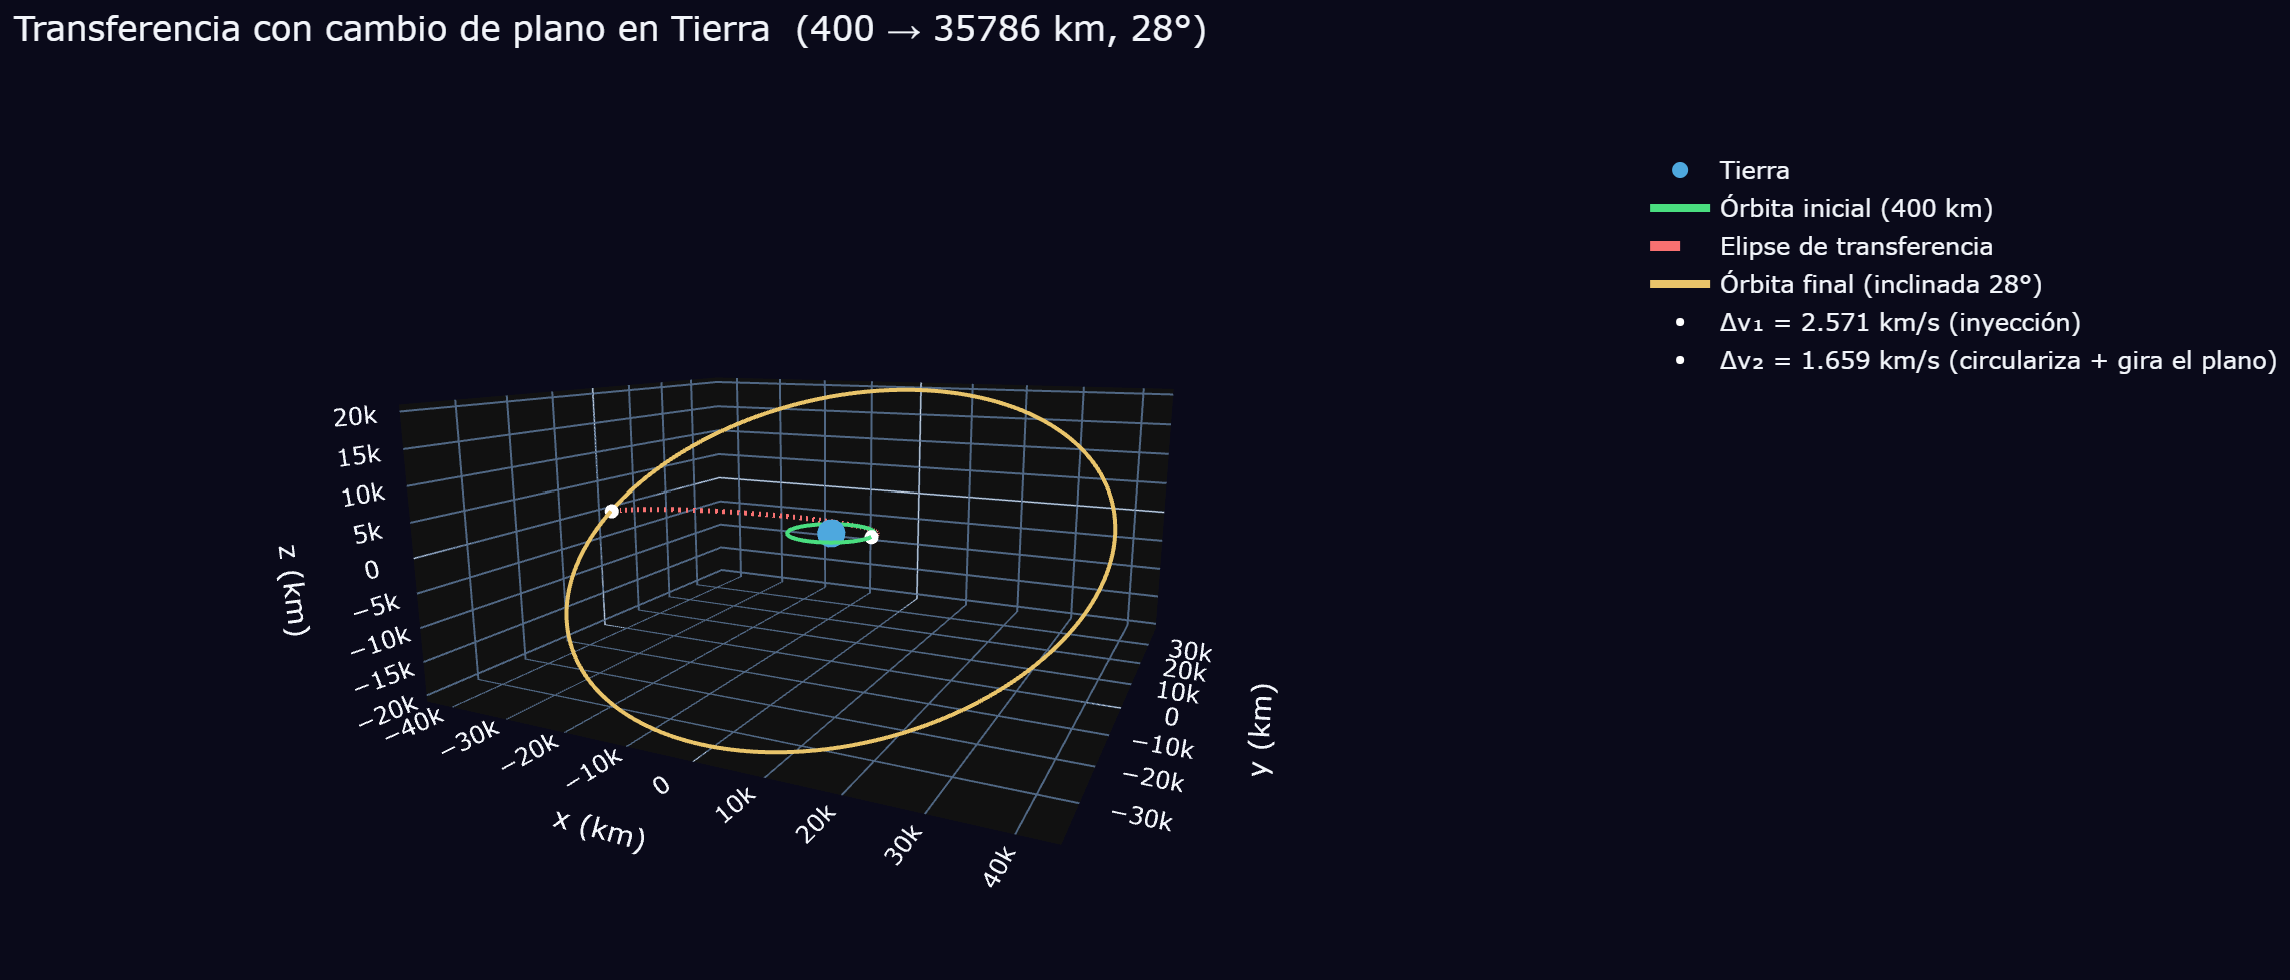
\includegraphics[width=0.95\textwidth]{tex/imagenes/llm_dibujo_cambio_plano.png}
  \caption{Figura generada por el asistente: vista tridimensional de la transferencia con
  cambio de plano, con la órbita final inclinada. Elaboración propia.}
  \label{fig:ap-llm-cambioplano-fig}
\end{figure}

\clearpage

% ---------------------------------------------------------------------------
\section{Aerofrenado}
\label{ap:llm-aerofrenado}

Ante una petición de rebajar una órbita aprovechando la atmósfera, el asistente invoca el
especialista de aerofrenado del cuerpo correspondiente y comunica el perigeo de operación, el
número de pasadas y la duración estimada (figura~\ref{fig:ap-llm-aero-chat}); la
figura~\ref{fig:ap-llm-aero-fig} es la curva de descenso del apogeo que dibuja a continuación.

\begin{figure}[htbp]
  \centering
  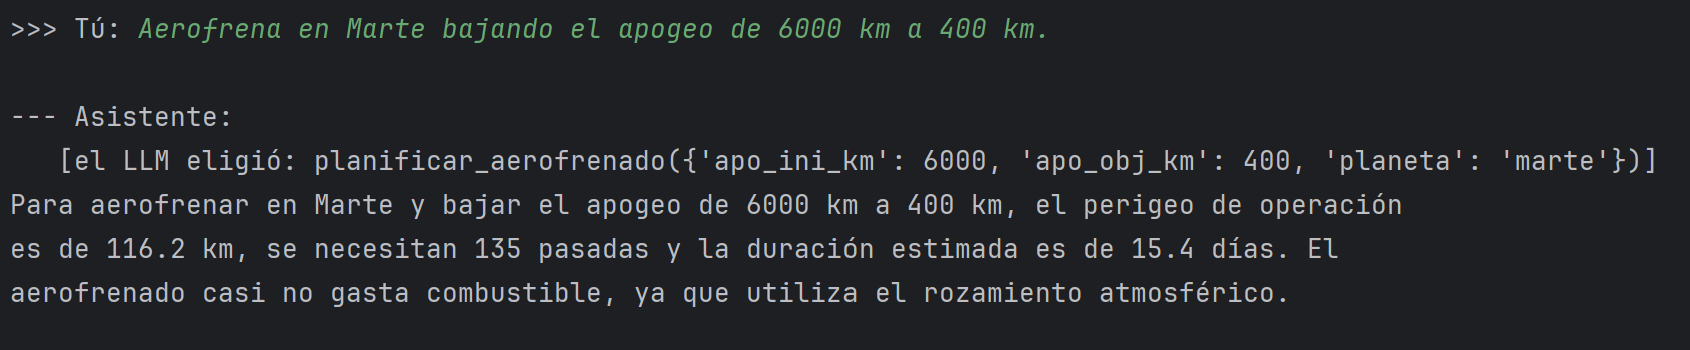
\includegraphics[width=0.9\textwidth]{tex/imagenes/llm_chat_aerofrenado.png}
  \caption{Conversación: el asistente planifica un aerofrenado en Marte. Elaboración propia.}
  \label{fig:ap-llm-aero-chat}
\end{figure}

\begin{figure}[htbp]
  \centering
  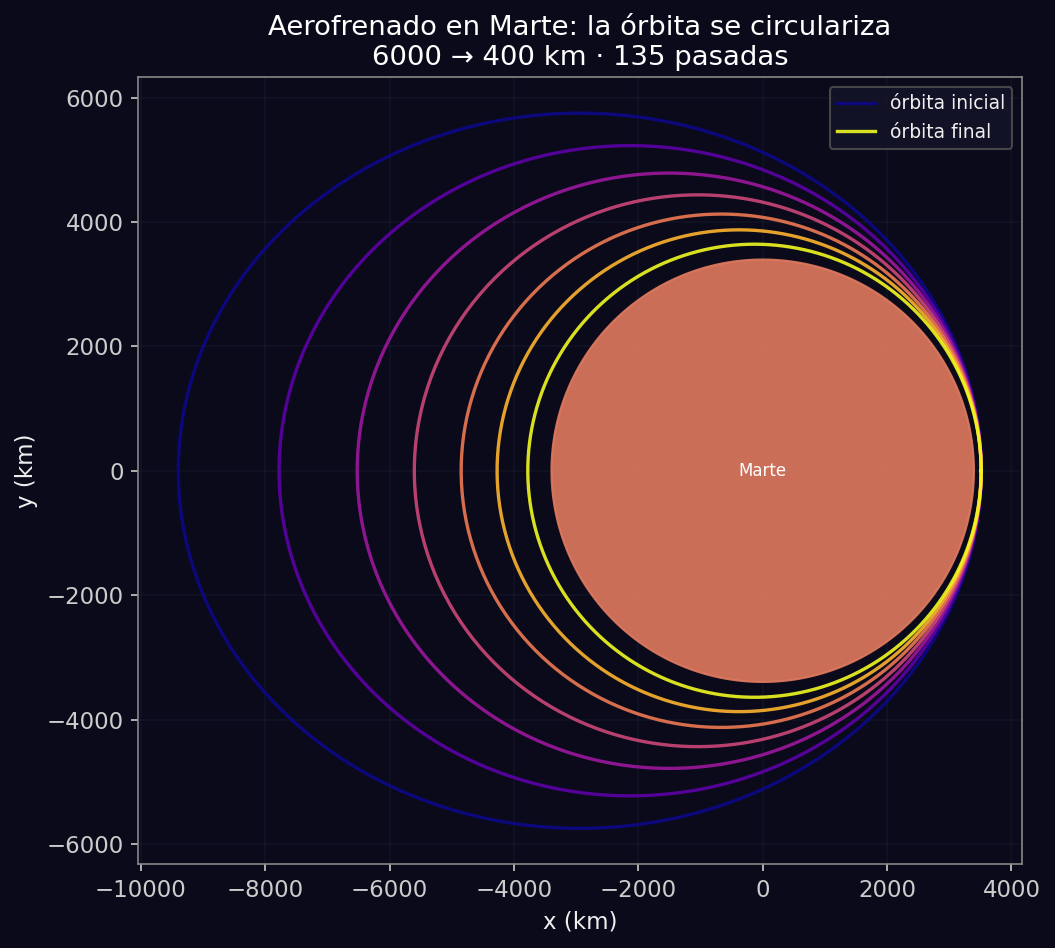
\includegraphics[width=0.82\textwidth]{tex/imagenes/llm_dibujo_aerofrenado.png}
  \caption{Figura generada por el asistente: descenso del apogeo pasada a pasada durante el
  aerofrenado. Elaboración propia.}
  \label{fig:ap-llm-aero-fig}
\end{figure}

\clearpage

% ---------------------------------------------------------------------------
\section{Viaje interplanetario}
\label{ap:llm-interplanetaria}

Para un trayecto entre dos planetas, el asistente resuelve el problema de Lambert con las
posiciones reales de los cuerpos y devuelve el $\Delta v$ de salida y de llegada, la energía
característica $C_3$ y la fecha de llegada (figura~\ref{fig:ap-llm-inter-chat}). La
figura~\ref{fig:ap-llm-inter-fig} representa la trayectoria heliocéntrica correspondiente.

\begin{figure}[htbp]
  \centering
  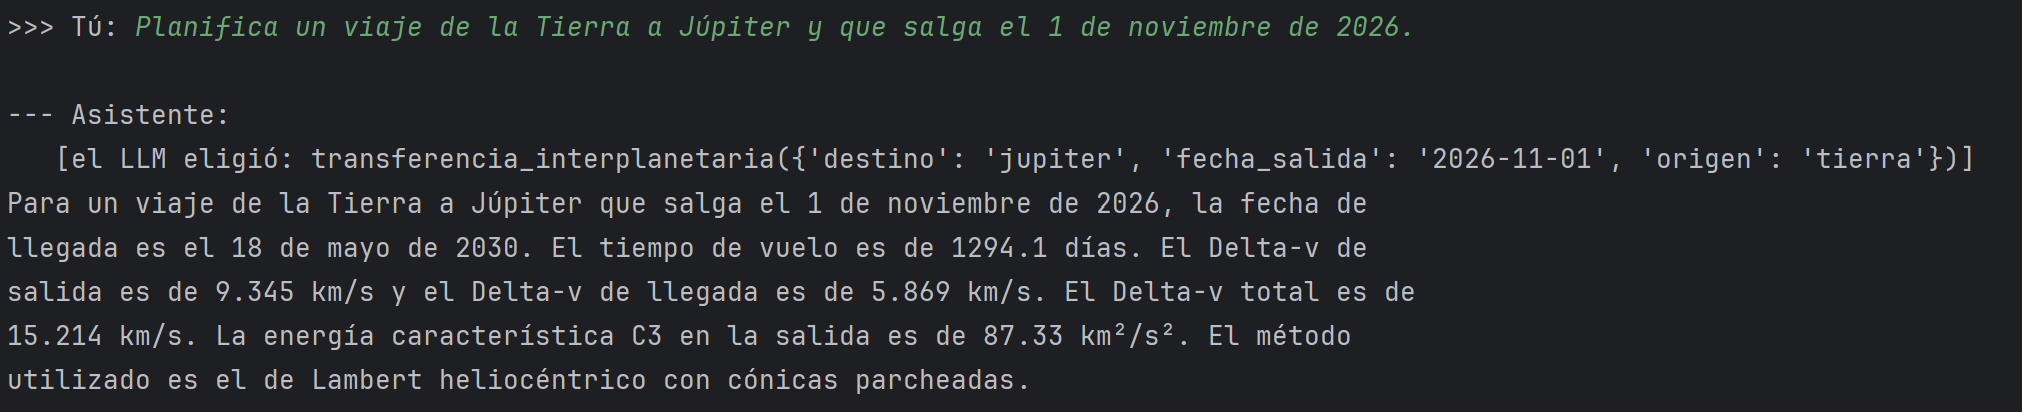
\includegraphics[width=0.9\textwidth]{tex/imagenes/llm_chat_interplanetaria.png}
  \caption{Conversación: el asistente calcula un viaje interplanetario Tierra--Marte.
  Elaboración propia.}
  \label{fig:ap-llm-inter-chat}
\end{figure}

\begin{figure}[htbp]
  \centering
  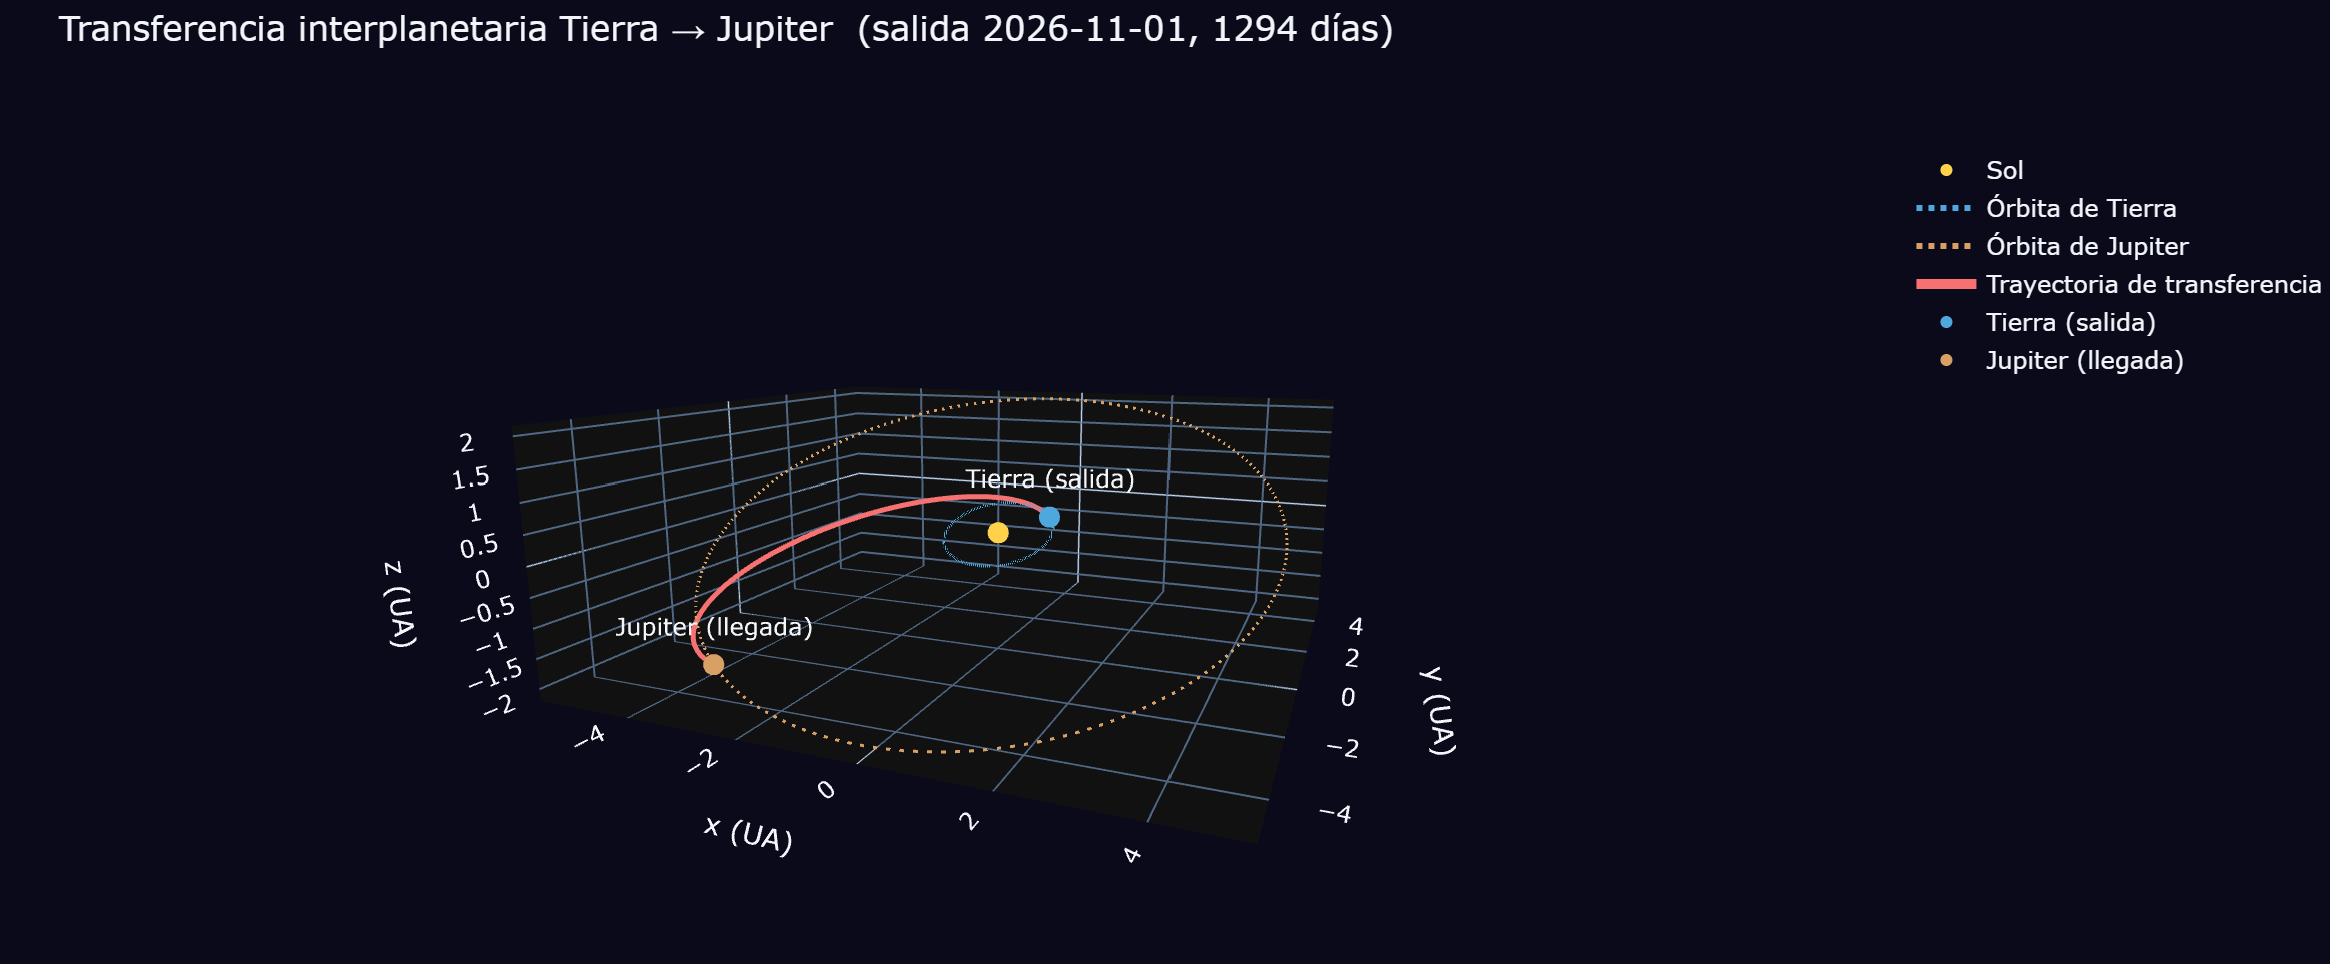
\includegraphics[width=0.95\textwidth]{tex/imagenes/llm_dibujo_interplanetaria.png}
  \caption{Figura generada por el asistente: trayectoria heliocéntrica del viaje entre la
  Tierra y Marte. Elaboración propia.}
  \label{fig:ap-llm-inter-fig}
\end{figure}

\clearpage

% ---------------------------------------------------------------------------
\section{Ventana de lanzamiento}
\label{ap:llm-porkchop}

Cuando la pregunta es por la mejor fecha para un viaje interplanetario, el asistente genera un
diagrama \textit{porkchop} y señala la ventana de mínimo coste. La
figura~\ref{fig:ap-llm-pork-chat} recoge la respuesta y la figura~\ref{fig:ap-llm-pork-fig},
el mapa de coste con la ventana óptima marcada.

\begin{figure}[htbp]
  \centering
  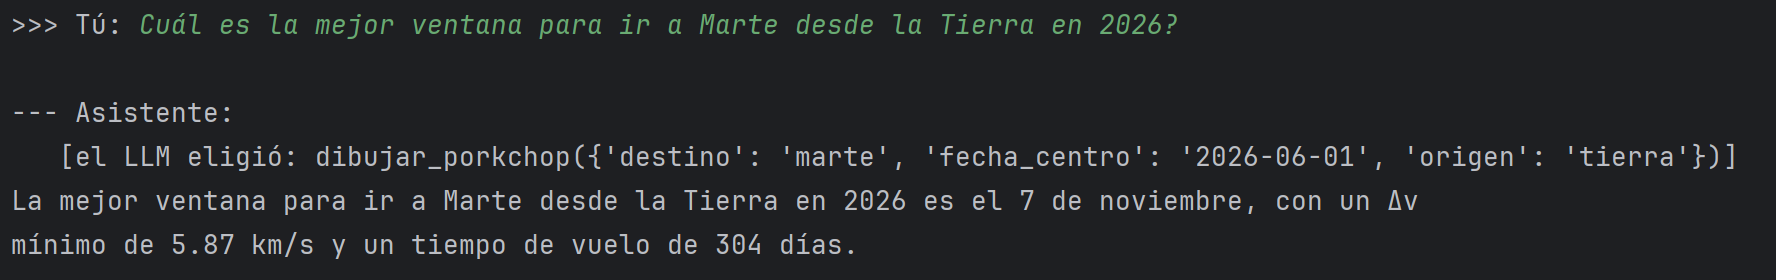
\includegraphics[width=0.9\textwidth]{tex/imagenes/llm_chat_porkchop.png}
  \caption{Conversación: el asistente determina la ventana de lanzamiento óptima
  Tierra--Marte. Elaboración propia.}
  \label{fig:ap-llm-pork-chat}
\end{figure}

\begin{figure}[htbp]
  \centering
  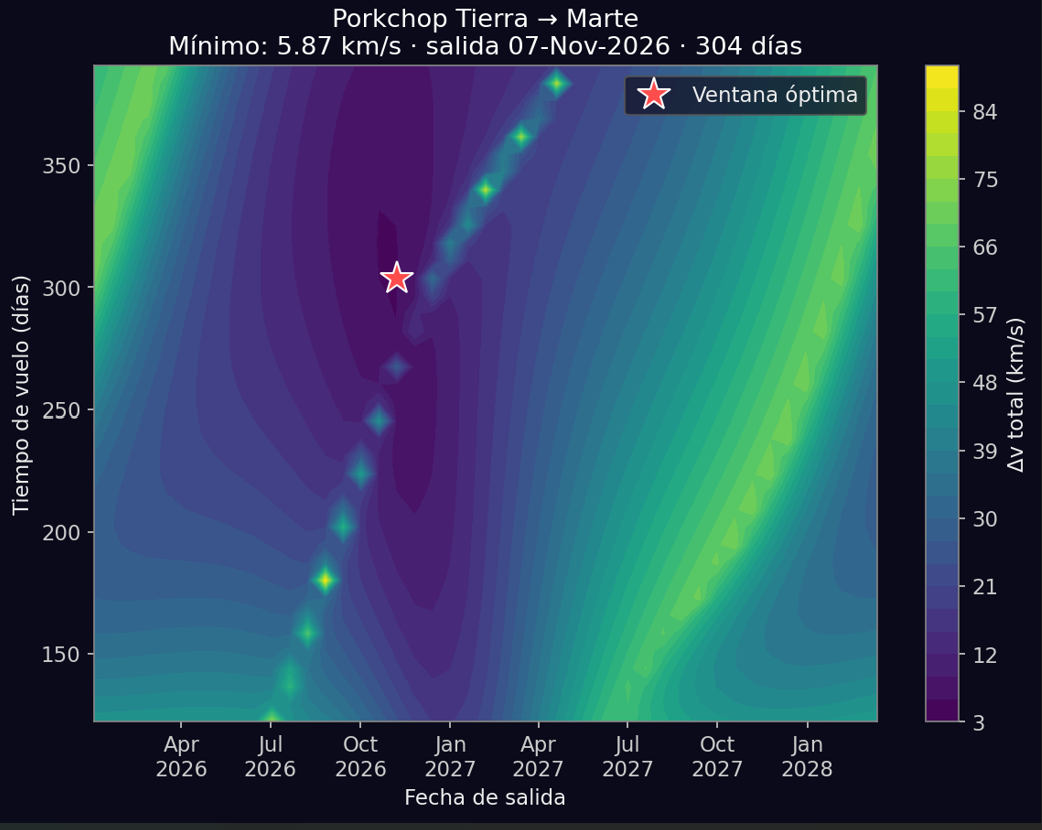
\includegraphics[width=0.88\textwidth]{tex/imagenes/llm_dibujo_porkchop.png}
  \caption{Figura generada por el asistente: diagrama \textit{porkchop} del viaje
  Tierra--Marte, con la ventana de mínimo coste marcada. Elaboración propia.}
  \label{fig:ap-llm-pork-fig}
\end{figure}